%%%%%%%%%%%%%%%%%%%%%%%%%%%%%%%%%%%%%%%%%
% Long Professional Curriculum Vitae
% LaTeX Template
% Version 1.1 (9/12/12)
%
% This template has been downloaded from:
% http://www.latextemplates.com
%
% Original author:
% Rensselaer Polytechnic Institute (http://www.rpi.edu/dept/arc/training/latex/resumes/)
%
% Important note:
% This template requires the res.cls file to be in the same directory as the
% .tex file. The res.cls file provides the resume style used for structuring the
% document.
%
%%%%%%%%%%%%%%%%%%%%%%%%%%%%%%%%%%%%%%%%%

%----------------------------------------------------------------------------------------
% PACKAGES AND OTHER DOCUMENT CONFIGURATIONS
%----------------------------------------------------------------------------------------

\let\nofiles\relax
\documentclass[12pt,a4paper]{res} % Use the res.cls style, the font size can be changed to 11pt or 12pt here

%\usepackage[utf8]{inputenc}
\usepackage[T1]{fontenc}
%\usepackage{helvet}
%\usepackage{ebgaramond}
%\usepackage{garamondx}
\usepackage{CormorantGaramond}

\usepackage{graphicx}
\usepackage[official]{eurosym}
\usepackage{wrapfig}
\usepackage{hyperref}
\usepackage{caption}
\captionsetup[figure]{labelformat=empty}

\usepackage[style=numeric,sorting=ydnt,defernumbers,maxbibnames=20]{biblatex}
% \addbibresource{publications.bib}
\AtEveryBibitem{\clearfield{url}}
\usepackage[usenames,dvipsnames,svgnames,table]{xcolor}
\definecolor{dark-gray}{gray}{0.2}
\newcommand{\sectionRule}{{\vspace{-6pt} \color{black} \hrulefill}}

\usepackage{longtable}

\newsectionwidth{0pt} % Stops section indenting

\pagestyle{plain}

\begin{document}

%----------------------------------------------------------------------------------------
% YOUR NAME AND ADDRESS(ES) SECTION
%----------------------------------------------------------------------------------------

\begin{figure}[htbp]
\begin{center}
%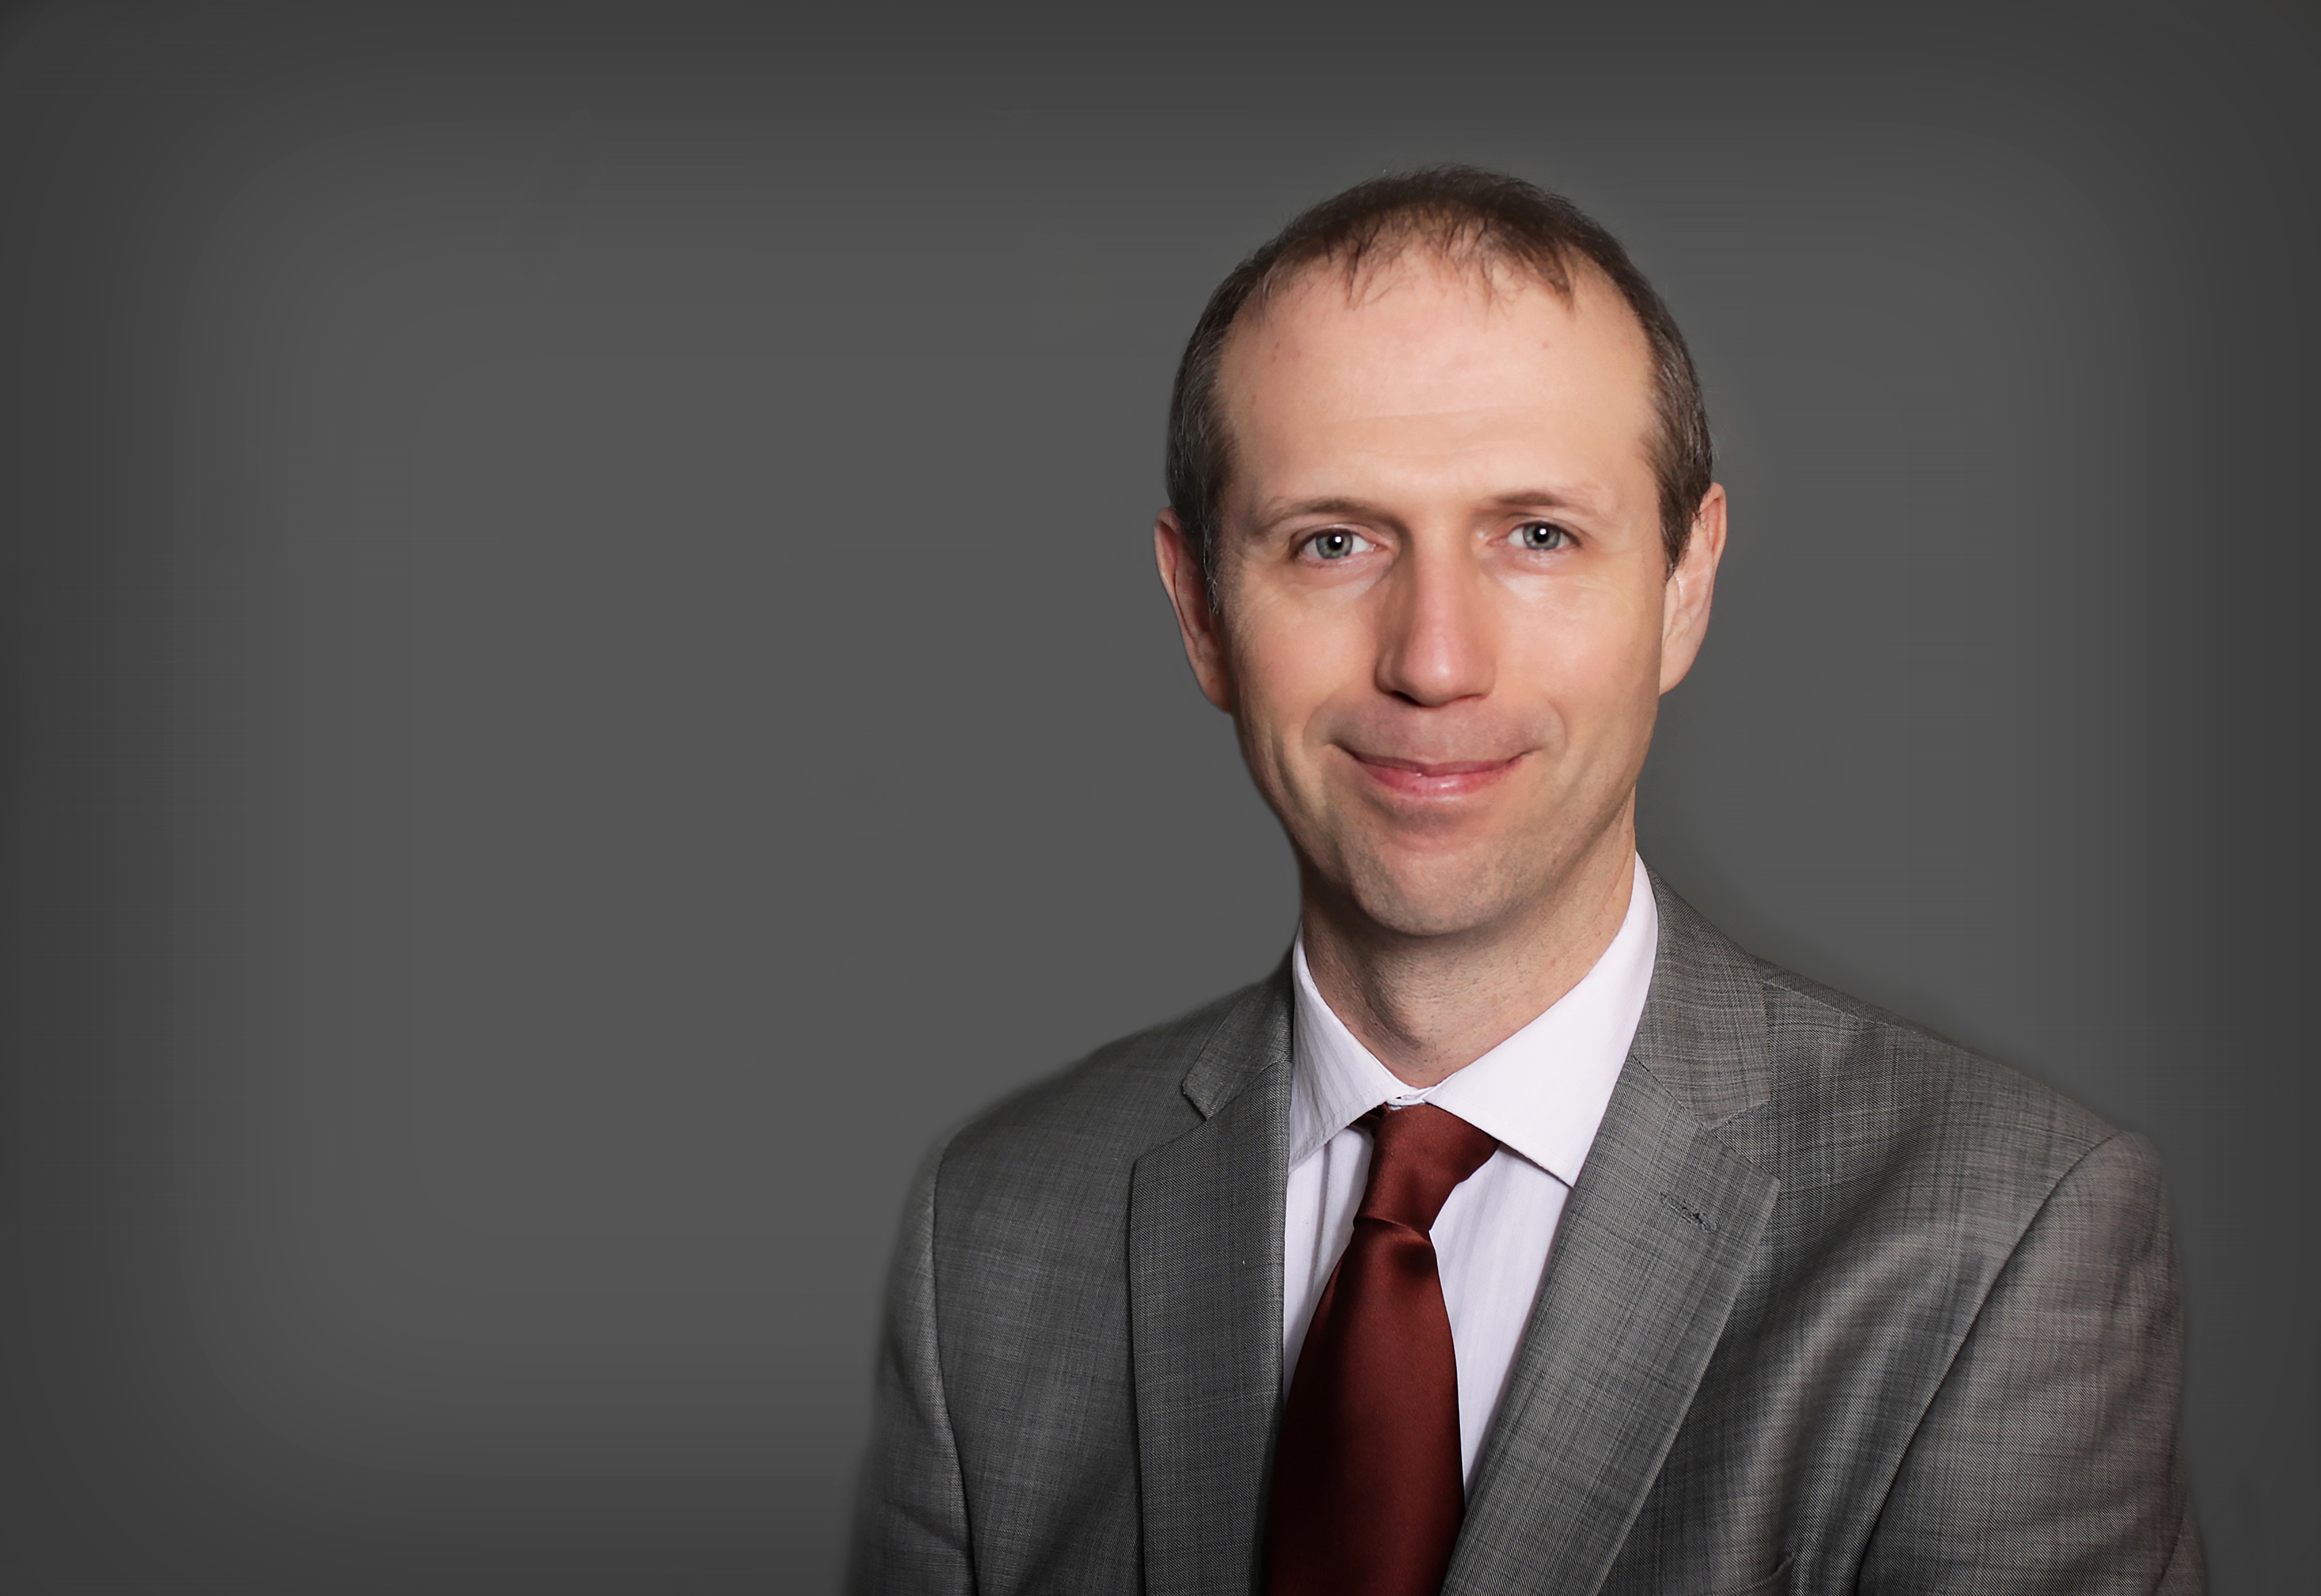
\includegraphics[width=0.125\textwidth]{figures/John.jpg}
\end{center}
\end{figure}

\name{Jacopo Uggeri} % Your name at the top

% If you don't want one of the addresses, simply remove all the text in the first or second \address{} bracket

\address{{\bf Address} \\ 134-136 Cromwell Road \\ SW74HA \\ London \\ United Kingdom} % Your address 1

\address{{\bf Contact} \\ \href{mailto:jacopo.uggeri@gmail.com}{jacopo.uggeri@gmail.com} \\ \url{github.com/jacopouggeri} \\ \url{youtube.com/@jacopouggeri}} % Your address 2

%----------------------------------------------------------------------------------------

\begin{resume}

%----------------------------------------------------------------------------------------
% OBJECTIVE SECTION
%----------------------------------------------------------------------------------------

\section{\centerline{Summary}}
\sectionRule
\vspace{6pt} % Gap between title and text

%----------------------------------------------------------------------------------------
% PROFESSIONAL EXPERIENCE SECTION
%----------------------------------------------------------------------------------------

\section{\centerline{Professional Experience}} 
\sectionRule
\vspace{6pt} % Gap between title and text

% \begin{itemize} \itemsep -2pt % Reduce space between items
% \end{itemize}

{\sl Graduate Teaching Assistant} \\
Department of Physics, Imperial College London (London), United Kingdom \hfill 2022 -- 2023

%----------------------------------------------------------------------------------------

% \vspace{0.2in} % Some whitespace between sections

%----------------------------------------------------------------------------------------
% EDUCATION SECTION
%----------------------------------------------------------------------------------------

\section{\centerline{Education}} 
\sectionRule
\vspace{6pt} % Gap between title and text

{\sl MSci Physics with Theoretical Physics}\\ 
Imperial College London (London), United Kingdom \hfill 2019 -- present

\begin{itemize} \itemsep -2pt
\item Undergraduate Integrated Masters programme in physics, attended a variety of courses that granted a solid foundation in scientific and critical thinking, with a focus on theoretical physics
\item Excellent academic performance, achieved 1st in theoretical modules: Mathematical Methods, Foundations of Quantum Mechanics, Advanced Classical Physics, Group Theory, Nuclear and Particle Physics, Statistical Mechanics
\item Current relevant courses: Quantum Field Theory, Unification, General Relativity, Cosmology
\item Used Python extensively for data analysis of experiments and simulations
\end{itemize}

{\sl Diploma di Laurea}\\ 
Imperial College London (London), United Kingdom \hfill 2019 -- present

\begin{itemize} \itemsep -2pt
\item Undergraduate Integrated Masters programme in physics, attended a variety of courses that granted a solid foundation in scientific and critical thinking, with a focus on theoretical physics
\item Excellent academic performance, achieved 1st in theoretical modules: Mathematical Methods, Foundations of Quantum Mechanics, Advanced Classical Physics, Group Theory, Nuclear and Particle Physics, Statistical Mechanics
\item Current relevant courses: Quantum Field Theory, Unification, General Relativity, Cosmology
\item Used Python extensively for data analysis of experiments and simulations
\end{itemize}



%----------------------------------------------------------------------------------------
 
% \vspace{0.2in} % Some whitespace between sections

%----------------------------------------------------------------------------------------
% RESEARCH SUMMARY SECTION
%----------------------------------------------------------------------------------------

\section{\centerline{Research Summary}}
\sectionRule
\subsection*{Research Interests}

\begin{itemize} \itemsep -2pt
\item Data Science; Artificial Intelligence; Social Semantics; Social Media; Semantic Web
\item Agricultural Technology; Smart Manufacturing; Innovation and Entrepreneurship
\item Electrical and Electronic Engineering; Power and Energy; Sensors and Internet of Things
\end{itemize}

\subsection*{Research Activity}

\begin{center}
Total refereed papers: \hfill 267 \\ % Check
Total books / book chapters: \hfill 8 / 19 \\ % Check
Total PhDs / Masters graduated: \hfill 14.5 / 6 \\
Total University of Galway funding as budget holder: \hfill \euro{}9,181,418 \\
Total University of Galway funding as PI / Co-PI: \hfill \euro{}46,622,884 \\
Current size of team: \hfill 14 (8.5 postgraduates; 5 postdocs; 1.5 lecturers; 0.5 admin) \\
Awards and honours: \hfill Best papers at IDCS, IoT, DL4KGS, SEMANTiCS, ICEGOV, ESWC, IEEE PELS \\
Journals reviewed for: \hfill 20 \\
Conference / workshop chairs: \hfill 5 / 20 \\
Conference / workshop programme committees: \hfill 40 / 30 \\
Other relevant indicators: \hfill Co-PI on the \euro{}49 million Insight Research Centre Phase 2 grant \\ \hfill Co-PI on the \euro{}25 million Confirm Research Centre grant \\ \hfill Co-PI on the \euro{}44 million Insight Research Centre grant \\ \hfill Co-PI on the \euro{}15 million DERI L\'{i}on II CSET grant \\ \hfill Project Leader for the \euro{}12 million DERI L\'{i}on I CSET grant from 2006 -- 2008
\end{center}

%----------------------------------------------------------------------------------------

\vspace{0.2in} % Some whitespace between sections

%----------------------------------------------------------------------------------------
\vspace{0.2in} % Some whitespace between sections

\end{resume} 
\end{document}